% ============================================================
%  Semaine 1 — Fondamentaux du web & environnement
%  PRÉSENTATION (Beamer) — cfpt·i | Anne Terrier
%  Charte graphique : cfpt·i (bleu accentBlue + jaune cfptYellow)
% ============================================================
\documentclass[aspectratio=169,11pt]{beamer}

\usepackage[T1]{fontenc}
\usepackage[utf8]{inputenc}
\usepackage[scaled=0.92]{helvet}
\renewcommand{\familydefault}{\sfdefault}

\usepackage{tikz}
\usetikzlibrary{positioning, arrows.meta, decorations.pathreplacing}
\usepackage{booktabs}
\usepackage{tabularx}
\usepackage{colortbl}
\usepackage{listings}

% ---------------------------------------------------------------
% Palette cfpt·i
% ---------------------------------------------------------------
\definecolor{cfptYellow}{HTML}{F5C400}
\definecolor{cfptBlack}{HTML}{1A1A1A}
\definecolor{cfptDarkGrey}{HTML}{555555}
\definecolor{cfptGrey}{HTML}{F2F2F2}
\definecolor{accentBlue}{HTML}{1D4E89}
\definecolor{lightBlue}{HTML}{D6E4F0}
\definecolor{codeGrey}{HTML}{F5F5F5}
\definecolor{successGreen}{HTML}{1E7145}
\definecolor{warningOrange}{HTML}{C55A11}

% Alias (repris du polycop)
\colorlet{uniInk}{cfptBlack}
\colorlet{uniNavy}{accentBlue}
\colorlet{uniTeal}{successGreen}
\colorlet{uniGold}{warningOrange}
\colorlet{uniGrey}{cfptDarkGrey}
\colorlet{uniPaper}{cfptGrey}
\colorlet{uniRule}{cfptDarkGrey!35}

% ---------------------------------------------------------------
% Thème Beamer personnalisé cfpt·i
% ---------------------------------------------------------------
\usetheme{default}
\usecolortheme{default}
\setbeamercolor{palette primary}{bg=accentBlue, fg=white}
\setbeamercolor{structure}{fg=accentBlue}
\setbeamercolor{frametitle}{bg=accentBlue, fg=white}
\setbeamercolor{title}{fg=white}
\setbeamercolor{block title}{bg=accentBlue, fg=white}
\setbeamercolor{block body}{bg=lightBlue!30, fg=cfptBlack}
\setbeamercolor{block title alerted}{bg=cfptYellow!85!black, fg=cfptBlack}
\setbeamercolor{block body alerted}{bg=cfptYellow!20, fg=cfptBlack}
\setbeamercolor{block title example}{bg=successGreen, fg=white}
\setbeamercolor{block body example}{bg=successGreen!8, fg=cfptBlack}
\setbeamercolor{itemize item}{fg=cfptYellow!85!black}
\setbeamercolor{itemize subitem}{fg=cfptDarkGrey}
\setbeamercolor{enumerate item}{fg=accentBlue}
\setbeamercolor{normal text}{fg=cfptBlack}
\setbeamercolor{footline}{fg=white}

\setbeamertemplate{itemize item}{\textbullet}
\setbeamertemplate{itemize subitem}{--}
\setbeamertemplate{navigation symbols}{}
\setbeamertemplate{blocks}[rounded][shadow=false]

% Titre de frame : bandeau plein largeur
\setbeamertemplate{frametitle}{%
  \nointerlineskip%
  \begin{beamercolorbox}[wd=\paperwidth, ht=2.6ex, dp=1.2ex, leftskip=0.3cm]{frametitle}%
    \usebeamerfont{frametitle}\bfseries\insertframetitle%
  \end{beamercolorbox}%
}

% Pied de page : logo texte + section + numéro
\setbeamertemplate{footline}{%
  \leavevmode%
  \hbox{%
    \begin{beamercolorbox}[wd=.32\paperwidth, ht=2.4ex, dp=1ex, leftskip=0.3cm]{palette primary}%
      \usebeamerfont{author in head/foot}\tiny Anne Terrier%
    \end{beamercolorbox}%
    \begin{beamercolorbox}[wd=.44\paperwidth, ht=2.4ex, dp=1ex, center]{palette primary}%
      \usebeamerfont{title in head/foot}\tiny Semaine 1 --- Fondamentaux du web%
    \end{beamercolorbox}%
    \begin{beamercolorbox}[wd=.24\paperwidth, ht=2.4ex, dp=1ex, right, rightskip=0.3cm]{palette primary}%
      \usebeamerfont{date in head/foot}\tiny\insertframenumber\,/\,\inserttotalframenumber%
    \end{beamercolorbox}%
  }%
}

% ---------------------------------------------------------------
% Listings
% ---------------------------------------------------------------
\lstset{
  basicstyle=\ttfamily\scriptsize,
  backgroundcolor=\color{codeGrey},
  frame=single, framerule=0.4pt,
  rulecolor=\color{cfptDarkGrey!40},
  breaklines=true,
  keywordstyle=\color{accentBlue}\bfseries,
  commentstyle=\color{cfptDarkGrey}\itshape,
  stringstyle=\color{successGreen},
  showstringspaces=false,
}



% ---------------------------------------------------------------
% Métadonnées
% ---------------------------------------------------------------
\title{Fondamentaux du web \& environnement}
\subtitle{Développement web --- Classe passerelle}
\author{Anne Terrier}
\institute{cfpt\textperiodcentered i --- École d'informatique}
\date{Semaine 1}

% ===============================================================
\begin{document}
% ===============================================================

% --- Diapo de titre ---
{
\setbeamertemplate{footline}{}
\begin{frame}[plain]
  \begin{tikzpicture}[remember picture, overlay]
    \fill[accentBlue] (current page.north west) rectangle ([yshift=-3.2cm]current page.north east);
    \node[anchor=north west, text=white, font=\huge\bfseries, text width=0.9\paperwidth]
      at ([shift={(0.8cm,-0.8cm)}]current page.north west)
      {Fondamentaux du web \& environnement};
    \node[anchor=north west, text=lightBlue, font=\large]
      at ([shift={(0.85cm,-2.55cm)}]current page.north west)
      {Développement web --- Classe passerelle};

    % accent jaune
    \fill[cfptYellow] ([yshift=-3.2cm]current page.north west) rectangle ([yshift=-3.35cm]current page.north east);

    \node[anchor=south west, font=\large\bfseries, text=accentBlue]
      at ([shift={(0.8cm,1.8cm)}]current page.south west) {Semaine 1};
    \node[anchor=south west, font=\normalsize, text=cfptDarkGrey]
      at ([shift={(0.8cm,1.1cm)}]current page.south west)
      {Anne Terrier \quad\textbar\quad cfpt\textperiodcentered i --- École d'informatique};
  \end{tikzpicture}
\end{frame}
}

% --- Plan ---
\begin{frame}{Au programme aujourd'hui}
  \begin{columns}[T]
    \begin{column}{0.48\textwidth}
      \begin{enumerate}
        \item Comment fonctionne le web ?
        \item Les langages côté client
        \item Les langages côté serveur
        \item La stack du cours
      \end{enumerate}
    \end{column}
    \begin{column}{0.48\textwidth}
      \begin{enumerate}
        \setcounter{enumi}{4}
        \item Environnement de développement
        \item Git --- premiers pas
      \end{enumerate}
      \vspace{0.6cm}
      \begin{block}{Objectif de la semaine}
        Comprendre le fonctionnement du web et installer son environnement de développement.
      \end{block}
    \end{column}
  \end{columns}
\end{frame}

% ===============================================================
\section{Comment fonctionne le web ?}
% ===============================================================
{
\setbeamertemplate{footline}{}
\begin{frame}[plain]
  \begin{tikzpicture}[remember picture, overlay]
    \fill[accentBlue] (current page.north west) rectangle (current page.south east);
    \fill[cfptYellow] ([yshift=-0.15cm]current page.center -| current page.west)
      rectangle ([yshift=-0.3cm]current page.center -| current page.east);
    \node[text=white, font=\Huge\bfseries] at ([yshift=0.9cm]current page.center)
      {1. Comment fonctionne le web ?};
  \end{tikzpicture}
\end{frame}
}

\begin{frame}{Le modèle client / serveur}
  \begin{center}
  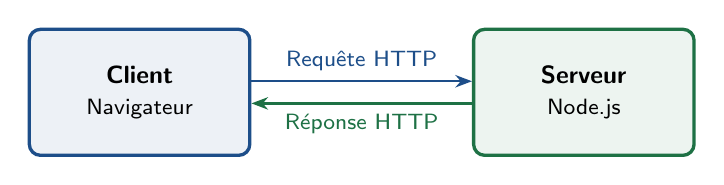
\begin{tikzpicture}[font=\small, node distance=2.8cm]
    \node[draw=accentBlue, very thick, rounded corners, fill=accentBlue!8,
          minimum width=2.8cm, minimum height=1.6cm, align=center] (client)
      {\textbf{Client}\\{\footnotesize Navigateur}};
    \node[draw=successGreen, very thick, rounded corners, fill=successGreen!8,
          minimum width=2.8cm, minimum height=1.6cm, align=center,
          right=of client] (server)
      {\textbf{Serveur}\\{\footnotesize Node.js}};
    \draw[-{Stealth[length=6pt]}, accentBlue, thick]
      ([yshift=4pt]client.east) -- node[above, font=\footnotesize]{Requête HTTP} ([yshift=4pt]server.west);
    \draw[-{Stealth[length=6pt]}, successGreen, thick]
      ([yshift=-4pt]server.west) -- node[below, font=\footnotesize]{Réponse HTTP} ([yshift=-4pt]client.east);
  \end{tikzpicture}
  \end{center}
    \vspace{0.5cm}
  \begin{block}{Définition --- Client et serveur}
    \textbf{Client} : programme qui \textit{demande} une ressource (le navigateur).\\
    \textbf{Serveur} : programme qui \textit{répond} en envoyant fichiers ou données.\\
    Communication via le protocole \textbf{HTTP} (ou \textbf{HTTPS} sécurisé).
  \end{block}
\end{frame}

\begin{frame}{Le modèle client / serveur --- en détail}
  \begin{center}
    
\includegraphics[width=0.9\textwidth]{Semaine1/images/client serveur.jpg}
  \end{center}  
\end{frame}

\begin{frame}{Anatomie d'une URL}
  \vspace{0.4cm}
  \begin{center}
  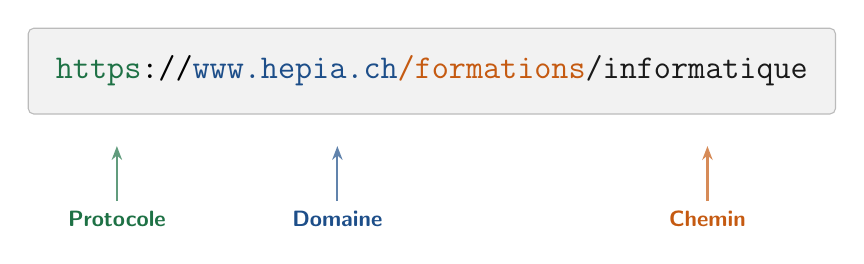
\begin{tikzpicture}[font=\small]
    \node[fill=cfptGrey, draw=cfptDarkGrey!40, thin, rounded corners=2pt, inner sep=10pt] (url)
      {\ttfamily\large
        \textcolor{successGreen}{https}://%
        \textcolor{accentBlue}{www.hepia.ch}%
        \textcolor{warningOrange}{/formations}%
        \textcolor{cfptBlack}{/informatique}};
    \node[below=1.1cm of url, xshift=-4cm, text=successGreen, font=\footnotesize\bfseries] (lp) {Protocole};
    \node[below=1.1cm of url, xshift=-1.2cm, text=accentBlue, font=\footnotesize\bfseries] (ld) {Domaine};
    \node[below=1.1cm of url, xshift=3.5cm, text=warningOrange, font=\footnotesize\bfseries] (lc) {Chemin};
    \draw[-{Stealth[length=5pt]}, successGreen!70, thick] (lp.north) -- ++(0,0.7);
    \draw[-{Stealth[length=5pt]}, accentBlue!70, thick] (ld.north) -- ++(0,0.7);
    \draw[-{Stealth[length=5pt]}, warningOrange!70, thick] (lc.north) -- ++(0,0.7);
  \end{tikzpicture}
  \end{center}
\end{frame}

\begin{frame}{DNS --- de l'adresse au nom}
  Un ordinateur ne comprend pas \texttt{www.hepia.ch} : il lui faut une \textbf{adresse IP} (ex. \texttt{192.0.2.34}). Le \textbf{DNS} traduit le nom de domaine en adresse IP.
  \vspace{0.3cm}
  \begin{block}{Analogie --- L'annuaire téléphonique}
    Tu connais le \textit{nom} (le domaine), l'annuaire te donne le \textit{numéro} (l'IP), et c'est ce numéro qui permet la communication.
  \end{block}
  \vspace{0.2cm}
  \textbf{Étapes simplifiées :}
  \begin{enumerate}
    \item Le navigateur demande : « quelle est l'IP de \texttt{www.hepia.ch} ? »
    \item Le serveur DNS répond avec l'adresse IP
    \item Le navigateur envoie sa requête HTTP à cette adresse
  \end{enumerate}
\end{frame}

\begin{frame}{Les codes de statut HTTP}
  \vspace{0.3cm}
  \begin{center}
  \begin{tabular}{cc>{\raggedright\arraybackslash}m{5cm}}
    \toprule
    \rowcolor{accentBlue}
    \color{white}\textbf{Code} & \color{white}\textbf{Signification} & \color{white}\textbf{Quand ?} \\
    \midrule
    \rowcolor{cfptGrey}
    \texttt{200} & OK & Tout s'est bien passé \\
    \texttt{301} & Redirection & La page a changé d'adresse \\
    \rowcolor{cfptGrey}
    \texttt{404} & Not Found & La page n'existe pas \\
    \texttt{500} & Server Error & Erreur côté serveur \\
    \bottomrule
  \end{tabular}
  \end{center}
  \vspace{0.3cm}
  \begin{center}
    \small\itshape Le fameux « 404 » que tout le monde a déjà rencontré !
  \end{center}
\end{frame}

\begin{frame}{Sites statiques et sites dynamiques}
  \small
  \begin{block}{Définition}
    \textbf{Statique} : renvoie toujours le même contenu (fichier HTML déjà prêt).\\
    \textbf{Dynamique} : génère le contenu à la demande, souvent depuis une base de données.
  \end{block}
  \vspace{0.1cm}
  \begin{center}
  \begin{tabularx}{\textwidth}{lXX}
    \toprule
    \rowcolor{accentBlue}
    \color{white}\textbf{} & \color{white}\textbf{Statique} & \color{white}\textbf{Dynamique} \\
    \midrule
    \rowcolor{cfptGrey}
    Contenu & Identique pour tous & Généré à chaque requête \\
    Exemple & Vitrine, portfolio & Forum, boutique, réseau social \\
    \rowcolor{cfptGrey}
    Technique & HTML/CSS/JS seuls & Node.js + base de données \\
    \bottomrule
  \end{tabularx}
  \end{center}
  \vspace{0.1cm}
  \begin{alertblock}{Où se situe MiniForum ?}
    Statique au départ (sem. 1--5), puis dynamique dès la phase 3 avec une vraie base de données.
  \end{alertblock}
\end{frame}

% ===============================================================
\section{Les langages côté client}
% ===============================================================
{
\setbeamertemplate{footline}{}
\begin{frame}[plain]
  \begin{tikzpicture}[remember picture, overlay]
    \fill[accentBlue] (current page.north west) rectangle (current page.south east);
    \fill[cfptYellow] ([yshift=-0.15cm]current page.center -| current page.west)
      rectangle ([yshift=-0.3cm]current page.center -| current page.east);
    \node[text=white, font=\Huge\bfseries] at ([yshift=0.9cm]current page.center)
      {2. Les langages côté client};
  \end{tikzpicture}
\end{frame}
}

\begin{frame}{HTML, CSS, JavaScript}
  \begin{center}
  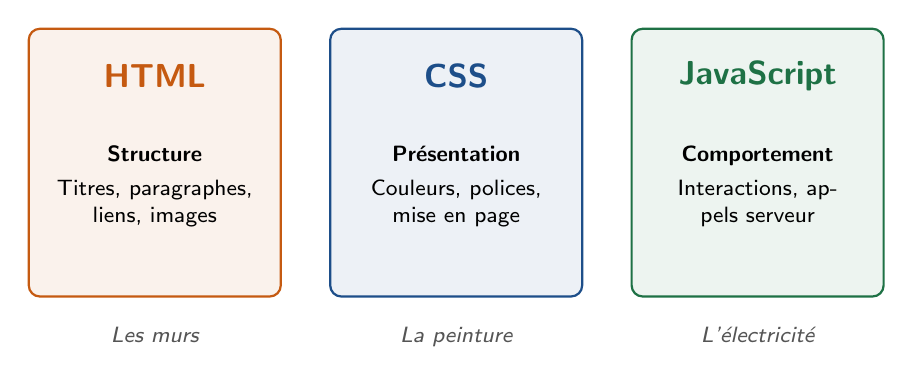
\begin{tikzpicture}[font=\small]
    \node[draw=warningOrange, thick, rounded corners, fill=warningOrange!8,
          minimum width=3.2cm, minimum height=3.4cm, align=center] (html) at (0,0) {};
    \node[font=\bfseries\large, text=warningOrange] at ([yshift=1.1cm]html.center) {HTML};
    \node[align=center, text width=2.9cm, font=\footnotesize] at ([yshift=-0.3cm]html.center)
      {\textbf{Structure}\\[3pt] Titres, paragraphes, liens, images};

    \node[draw=accentBlue, thick, rounded corners, fill=accentBlue!8,
          minimum width=3.2cm, minimum height=3.4cm, align=center,
          right=0.6cm of html] (css) {};
    \node[font=\bfseries\large, text=accentBlue] at ([yshift=1.1cm]css.center) {CSS};
    \node[align=center, text width=2.9cm, font=\footnotesize] at ([yshift=-0.3cm]css.center)
      {\textbf{Présentation}\\[3pt] Couleurs, polices, mise en page};

    \node[draw=successGreen, thick, rounded corners, fill=successGreen!8,
          minimum width=3.2cm, minimum height=3.4cm, align=center,
          right=0.6cm of css] (js) {};
    \node[font=\bfseries\large, text=successGreen] at ([yshift=1.1cm]js.center) {JavaScript};
    \node[align=center, text width=2.9cm, font=\footnotesize] at ([yshift=-0.3cm]js.center)
      {\textbf{Comportement}\\[3pt] Interactions, appels serveur};

    \node[below=0.25cm of html.south, font=\footnotesize\itshape, text=cfptDarkGrey] {Les murs};
    \node[below=0.25cm of css.south, font=\footnotesize\itshape, text=cfptDarkGrey] {La peinture};
    \node[below=0.25cm of js.south, font=\footnotesize\itshape, text=cfptDarkGrey] {L'électricité};
  \end{tikzpicture}
  \end{center}
  \begin{alertblock}{Qui exécute quoi ?}
    HTML, CSS et JavaScript s'exécutent dans le \textbf{navigateur} (côté client).
  \end{alertblock}
\end{frame}

\begin{frame}[fragile]{Un premier exemple --- la structure (HTML)}
\begin{lstlisting}[language=HTML]
<!DOCTYPE html>
<html lang="fr">
<head>
  <meta charset="UTF-8">
  <title>MiniForum</title>
  <link rel="stylesheet" href="style.css">
</head>
<body>
  <h1>Bienvenue sur MiniForum</h1>
  <button id="btn">Cliquez-moi</button>
  <script src="app.js"></script>
</body>
</html>
\end{lstlisting}
\end{frame}

\begin{frame}[fragile]{Un premier exemple --- présentation \& comportement}
  \begin{columns}[T]
    \begin{column}{0.5\textwidth}
      \begin{center}\footnotesize\textbf{style.css}\end{center}
\begin{lstlisting}[language=HTML]
button {
  background-color: #1D3557;
  color: white;
  padding: 10px 20px;
  border: none;
  border-radius: 4px;
  cursor: pointer;
}
\end{lstlisting}
    \end{column}
    \begin{column}{0.5\textwidth}
      \begin{center}\footnotesize\textbf{app.js}\end{center}
\begin{lstlisting}[language=bash]
const btn =
  document.getElementById('btn');

btn.addEventListener('click',
  () => {
    alert('Bonjour depuis JS !');
  });
\end{lstlisting}
    \end{column}
  \end{columns}
  \vspace{0.3cm}
  \begin{center}
    \small HTML \textbf{structure}, CSS \textbf{habille}, JavaScript \textbf{anime}.
  \end{center}
\end{frame}

% ===============================================================
\section{Les langages côté serveur}
% ===============================================================
{
\setbeamertemplate{footline}{}
\begin{frame}[plain]
  \begin{tikzpicture}[remember picture, overlay]
    \fill[accentBlue] (current page.north west) rectangle (current page.south east);
    \fill[cfptYellow] ([yshift=-0.15cm]current page.center -| current page.west)
      rectangle ([yshift=-0.3cm]current page.center -| current page.east);
    \node[text=white, font=\Huge\bfseries] at ([yshift=0.9cm]current page.center)
      {3. Les langages côté serveur};
  \end{tikzpicture}
\end{frame}
}

\begin{frame}{Côté serveur : un choix de langages}
  \begin{block}{Dans ce cours}
    \textbf{Node.js} s'exécute sur le \textbf{serveur}. La base de données est aussi côté serveur, jamais accessible directement depuis le navigateur.
  \end{block}
  \begin{exampleblock}{Pour info --- D'autres langages, mêmes principes}
    Contrairement au navigateur, un serveur n'est pas limité à un seul langage : \textbf{PHP, Python, Java, Ruby, C\#}... coexistent sur le web. Chacun peut jouer le même rôle que Node.js.
    \vspace{0.2cm}

    Le principe reste partout le même : recevoir une requête, dialoguer avec une base de données (en \textbf{SQL}), renvoyer une réponse.
  \end{exampleblock}
\end{frame}

% ===============================================================
\section{La stack du cours}
% ===============================================================
{
\setbeamertemplate{footline}{}
\begin{frame}[plain]
  \begin{tikzpicture}[remember picture, overlay]
    \fill[accentBlue] (current page.north west) rectangle (current page.south east);
    \fill[cfptYellow] ([yshift=-0.15cm]current page.center -| current page.west)
      rectangle ([yshift=-0.3cm]current page.center -| current page.east);
    \node[text=white, font=\Huge\bfseries] at ([yshift=0.9cm]current page.center)
      {4. La stack du cours};
  \end{tikzpicture}
\end{frame}
}

\begin{frame}{La stack de MiniForum}
  \begin{center}
  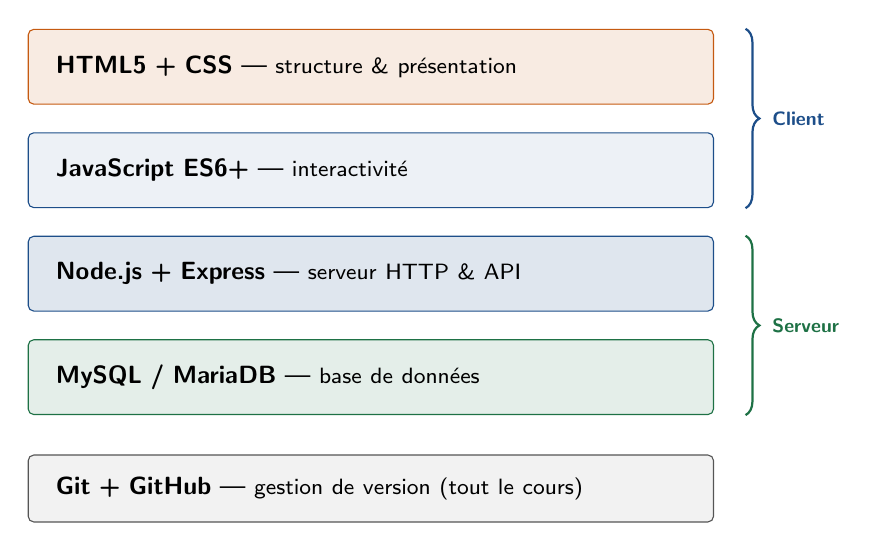
\begin{tikzpicture}[font=\small, node distance=0.35cm,
    layer/.style={draw=cfptDarkGrey, thin, rounded corners=2pt, text width=8cm,
      minimum height=0.95cm, align=left, inner xsep=10pt}]
    \node[layer, fill=warningOrange!12, draw=warningOrange] (html)
      {\textbf{HTML5 + CSS} --- {\footnotesize structure \& présentation}};
    \node[layer, fill=accentBlue!8, draw=accentBlue, below=of html] (js)
      {\textbf{JavaScript ES6+} --- {\footnotesize interactivité}};
    \node[layer, fill=accentBlue!14, draw=accentBlue, below=of js] (node)
      {\textbf{Node.js + Express} --- {\footnotesize serveur HTTP \& API}};
    \node[layer, fill=successGreen!12, draw=successGreen, below=of node] (sql)
      {\textbf{MySQL / MariaDB} --- {\footnotesize base de données}};

    \draw[decorate, decoration={brace,amplitude=5pt}, accentBlue, thick]
      ([xshift=0.4cm]html.north east) -- ([xshift=0.4cm]js.south east)
      node[midway, right=6pt, font=\scriptsize\bfseries, text=accentBlue]{Client};
    \draw[decorate, decoration={brace,amplitude=5pt}, successGreen, thick]
      ([xshift=0.4cm]node.north east) -- ([xshift=0.4cm]sql.south east)
      node[midway, right=6pt, font=\scriptsize\bfseries, text=successGreen]{Serveur};

    \node[layer, fill=cfptGrey, draw=cfptDarkGrey, minimum height=0.85cm, below=0.5cm of sql] (git)
      {\textbf{Git + GitHub} --- {\footnotesize gestion de version (tout le cours)}};
  \end{tikzpicture}
  \end{center}
\end{frame}

\begin{frame}{À retenir}
  \begin{block}{Une application web = trois parties}
    \begin{itemize}
      \item une interface \textbf{côté client}
      \item un serveur \textbf{côté serveur}
      \item une \textbf{base de données}
    \end{itemize}
  \end{block}
  \vspace{0.3cm}
  \begin{exampleblock}{La particularité de ce cours}
    Nous utiliserons \textbf{JavaScript des deux côtés} : dans le navigateur \emph{et} sur le serveur (Node.js). Un seul langage à maîtriser pour toute la stack applicative.
  \end{exampleblock}
\end{frame}

% ===============================================================
\section{Environnement de développement}
% ===============================================================
{
\setbeamertemplate{footline}{}
\begin{frame}[plain]
  \begin{tikzpicture}[remember picture, overlay]
    \fill[accentBlue] (current page.north west) rectangle (current page.south east);
    \fill[cfptYellow] ([yshift=-0.15cm]current page.center -| current page.west)
      rectangle ([yshift=-0.3cm]current page.center -| current page.east);
    \node[text=white, font=\Huge\bfseries] at ([yshift=0.9cm]current page.center)
      {5. Environnement de développement};
  \end{tikzpicture}
\end{frame}
}

\begin{frame}{Les outils à installer}
  \begin{columns}[T]
    \begin{column}{0.5\textwidth}
      \begin{block}{À installer cette semaine}
        \begin{itemize}
          \item \textbf{VS Code} --- éditeur de code
          \item \textbf{Node.js} (LTS) --- serveur JS
          \item \textbf{Git} --- gestion de version
          \item Un compte \textbf{GitHub}
        \end{itemize}
      \end{block}
    \end{column}
    \begin{column}{0.5\textwidth}
      \begin{exampleblock}{Extensions VS Code}
        \begin{itemize}
          \item Prettier --- mise en forme
          \item ESLint --- qualité du code
          \item Live Server --- aperçu live
          \item GitLens --- visualiser Git
        \end{itemize}
      \end{exampleblock}
    \end{column}
  \end{columns}
  \vspace{0.3cm}
  \begin{center}
    \small Le détail pas-à-pas se trouve dans la \textbf{fiche TP} de la semaine.
  \end{center}
\end{frame}

\begin{frame}[fragile]{Premiers pas dans le terminal}
\begin{lstlisting}[language=bash]
pwd           # afficher le dossier courant
ls            # lister les fichiers
cd miniforum  # entrer dans un dossier
cd ..         # remonter d'un niveau
mkdir css     # creer un dossier
touch app.js  # creer un fichier vide
\end{lstlisting}
  \vspace{0.2cm}
  \begin{center}
    \small Ces commandes seront approfondies dans le cours \textbf{Linux / Bash}.
  \end{center}
\end{frame}

% ===============================================================
\section{Git --- premiers pas}
% ===============================================================
{
\setbeamertemplate{footline}{}
\begin{frame}[plain]
  \begin{tikzpicture}[remember picture, overlay]
    \fill[accentBlue] (current page.north west) rectangle (current page.south east);
    \fill[cfptYellow] ([yshift=-0.15cm]current page.center -| current page.west)
      rectangle ([yshift=-0.3cm]current page.center -| current page.east);
    \node[text=white, font=\Huge\bfseries] at ([yshift=0.9cm]current page.center)
      {6. Git --- premiers pas};
  \end{tikzpicture}
\end{frame}
}

\begin{frame}{Pourquoi utiliser Git ?}
  \begin{itemize}
    \item \textbf{Sauvegarder} son travail et son historique
    \item \textbf{Revenir en arrière} en cas d'erreur
    \item \textbf{Collaborer} à plusieurs sans s'écraser
    \item \textbf{Partager} son code (GitHub)
  \end{itemize}
  \vspace{0.4cm}
  \begin{block}{L'outil standard du métier}
    Git est utilisé par la quasi-totalité des équipes de développement dans le monde. Le maîtriser tôt est un vrai atout.
  \end{block}
\end{frame}

\begin{frame}{Les quatre zones de Git}
  \vspace{0.3cm}
  \begin{center}
  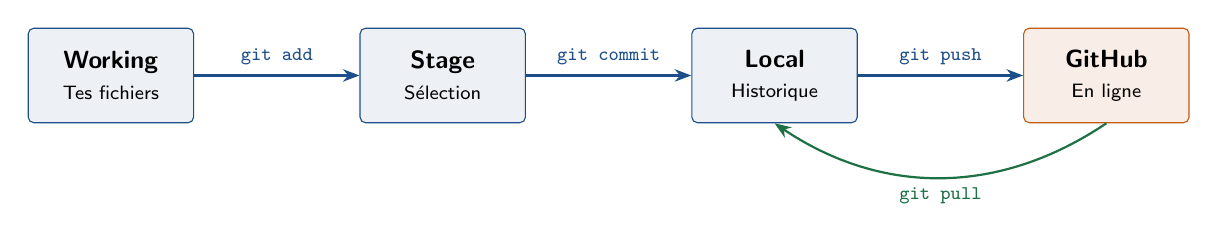
\begin{tikzpicture}[font=\small, node distance=2.1cm,
    state/.style={draw=accentBlue, thin, rounded corners=2pt, fill=accentBlue!8,
      minimum width=2.1cm, minimum height=1.2cm, align=center},
    remote/.style={draw=warningOrange, thin, rounded corners=2pt, fill=warningOrange!10,
      minimum width=2.1cm, minimum height=1.2cm, align=center},
    arr/.style={-{Stealth[length=6pt]}, thick}]
    \node[state] (wd) {\textbf{Working}\\{\scriptsize Tes fichiers}};
    \node[state, right=of wd] (st) {\textbf{Stage}\\{\scriptsize Sélection}};
    \node[state, right=of st] (lo) {\textbf{Local}\\{\scriptsize Historique}};
    \node[remote, right=of lo] (gh) {\textbf{GitHub}\\{\scriptsize En ligne}};
    \draw[arr, accentBlue] (wd) -- node[above, font=\scriptsize]{\texttt{git add}} (st);
    \draw[arr, accentBlue] (st) -- node[above, font=\scriptsize]{\texttt{git commit}} (lo);
    \draw[arr, accentBlue] (lo) -- node[above, font=\scriptsize]{\texttt{git push}} (gh);
    \draw[arr, successGreen, bend right=-34] (gh.south) to node[below, font=\scriptsize]{\texttt{git pull}} (lo.south);
  \end{tikzpicture}
  \end{center}
  \begin{exampleblock}{Analogie --- La photo de groupe}
    \textbf{Working} : tout le monde est dans la salle. \textbf{Stage} : certains se placent. \textbf{Commit} : on prend la photo (instantané). \textbf{Push} : on l'envoie sur le serveur partagé.
  \end{exampleblock}
\end{frame}

\begin{frame}[fragile]{Commandes essentielles}
\begin{lstlisting}[language=bash]
git init                    # initialiser un depot
git status                  # etat des fichiers
git add .                   # tout ajouter au stage
git commit -m "message"     # enregistrer un commit
git push origin main        # envoyer sur GitHub
git pull                    # recuperer les changements
\end{lstlisting}
  \vspace{0.2cm}
  \begin{alertblock}{Le bon réflexe}
    Commit \textbf{souvent}, avec des messages clairs. Un commit = une étape logique de ton travail.
  \end{alertblock}
\end{frame}

% ===============================================================
% Clôture
% ===============================================================
\begin{frame}{Résumé de la semaine}
  \begin{columns}[T]
    \begin{column}{0.5\textwidth}
      \begin{block}{Ce qu'on a vu}
        \begin{itemize}
          \item Le web = client + serveur + HTTP
          \item URL, DNS, codes de statut
          \item Statique vs dynamique
          \item HTML / CSS / JS côté client
          \item La stack MiniForum
        \end{itemize}
      \end{block}
    \end{column}
    \begin{column}{0.5\textwidth}
      \begin{alertblock}{À faire pour la semaine 2}
        \begin{itemize}
          \item Installer les outils (fiche TP)
          \item Créer son dépôt GitHub
          \item Faire le quiz Moodle
        \end{itemize}
      \end{alertblock}
    \end{column}
  \end{columns}
\end{frame}

{
\setbeamertemplate{footline}{}
\begin{frame}[plain]
  \begin{tikzpicture}[remember picture, overlay]
    \fill[accentBlue] (current page.north west) rectangle (current page.south east);
    \node[text=white, font=\Huge\bfseries] at ([yshift=0.6cm]current page.center) {Des questions ?};
    \fill[cfptYellow] ([yshift=-0.2cm]current page.center -| current page.west)
      rectangle ([yshift=-0.32cm]current page.center -| current page.east);
    \node[text=lightBlue, font=\large] at ([yshift=-1.3cm]current page.center)
      {Prochaine étape : la fiche TP --- mise en place du projet};
  \end{tikzpicture}
\end{frame}
}

\end{document}
